%!TEX root = ../dokumentation.tex

\chapter{Musterkapitel}

Verwendung Akronyms: \acf{AGPL}. Zweite Erwähnung einer Abkürzung \ac{AGPL} (Erklärung wird nicht mehr angezeigt)

Verweise auf das Glossar: \gls{Glossareintrag}, \glspl{Glossareintrag}

Nur erwähnte Literaturverweise werden auch im Literaturverzeichnis gedruckt:
\cite{baumgartner:2002}, \cite{dreyfus:1980}

%Quelle muss in Fußnote stehen (da sonst aufgrund eines Fehlers nicht kompiliert wird)
Meine erste Fußnote\footnote{Ich bin eine Fußnote aus \cite{mustermann:2012}} Verweis auf den Code \autoref{Python-Code}

%language ändert die Sprache. (Wenn nur eine Sprache verwendet wird, kann diese Sprache in einstellungen.tex geändert werden. Standardmäßig Java.)
%title wird unter dem Bsp. abgedruckt, wenn title leer, dann Listing {Nummer}: caption
%caption wird im Verzeichnis abgedruckt
%label wird zum referenzieren benutzt, muss einzigartig sein.
\begin{lstlisting}[caption=Python-Code, label=Python-Code, language=Python]
def quicksort(liste):
if len(liste) <= 1:
	return liste
pivotelement = liste.pop()
links = [element for element in liste if element < pivotelement]
rechts = [element for element in liste if element >= pivotelement]
return quicksort(links) + [pivotelement] + quicksort(rechts)
# Quelle: http://de.wikipedia.org/wiki/Python_(Programmiersprache)
\end{lstlisting}

\section{lorem ipsum}

\begin{wrapfigure}{r}{.4\textwidth}
\centering
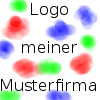
\includegraphics[height=.35\textwidth]{logo.png}
\vspace{-15pt}
\caption{Das Logo der Musterfirma\footnotemark}
\end{wrapfigure}

Looking for the one superhero comic you just have to read. Following the antics and adventures of May Mayday Parker, 
this Spider-book has everything you could want in a comic--action, laughs, mystery and someone in a Spidey suit. 
Collects Alias \#1-28, What If. Jessica Jones had Joined the Avengers. In her inaugural arc, Jessicas life immediately 
becomes expendable when she uncovers the potentially explosive secret of one heros true identity. 
Once upon a time, Jessica Jones was a costumed super-hero, just not a very good one. First, a story where Wolverine and 
Hulk come together, and then Captain America and Cable meet up.

